% ---------------------------------------------------------------
% TEMPLATE TCC1 - SENAC SANTO AMARO
% ---------------------------------------------------------------
% Trabalho de Conclusão de Curso 1
% Elaborado para apresentação da proposta inicial do TCC
% Estrutura: 4 capítulos (Introdução, Revisão Bibliográfica,
%            Desenvolvimento, Referências Bibliográficas)
% ---------------------------------------------------------------

\documentclass[
    12pt,                % tamanho da fonte
    openright,           % capítulos começam em página ímpar
    oneside,             % para impressão em apenas um lado do papel
    a4paper,             % tamanho do papel
    english,             % idioma adicional
    brazil               % idioma principal
]{abntex2}

% ---------------------------------------------------------------
% PACOTES
% ---------------------------------------------------------------
\usepackage{comment}                % Permite incluir trechos de código comentados
\usepackage{lmodern}                % Fonte Latin Modern
\usepackage[T1]{fontenc}            % Seleção de códigos de fonte
\usepackage[utf8]{inputenc}         % Codificação do documento
\usepackage{lastpage}               % Usado pela Ficha catalográfica
\usepackage{indentfirst}            % Indenta o primeiro parágrafo
\usepackage{color}                  % Controle de cores
\usepackage{graphicx}               % Inclusão de gráficos
\usepackage{microtype}              % Melhorias de justificação
\usepackage{float}                  % Para posicionamento de figuras
\usepackage{booktabs}               % Tabelas profissionais
\usepackage{multirow}               % Células mescladas em tabelas
\usepackage{longtable}              % Tabelas longas
\usepackage{amsmath,amssymb}        % Símbolos matemáticos
\usepackage{pgfgantt}               % Diagramas de Gantt
\usepackage[brazilian,hyperpageref]{backref}  % Páginas com citações
\usepackage[alf]{abntex2cite}       % Citações ABNT
\usepackage{caption}

% ---------------------------------------------------------------
% CONFIGURAÇÕES DO PDF
% ---------------------------------------------------------------
\makeatletter
\hypersetup{
    pdftitle={\@title},
    pdfauthor={\@author},
    pdfsubject={TCC1 - SENAC Santo Amaro},
    pdfcreator={LaTeX with abnTeX2},
    pdfkeywords={tcc}{senac}{santo amaro}{trabalho de conclusão},
    colorlinks=true,        % false: links em caixas; true: links coloridos
    linkcolor=blue,         % cor dos links internos
    citecolor=blue,         % cor dos links para bibliografia
    filecolor=magenta,      % cor dos links para arquivos
    urlcolor=blue,
    bookmarksdepth=4
}
\makeatother

% ---------------------------------------------------------------
% CONFIGURAÇÕES DE APARÊNCIA DO PDF FINAL
% ---------------------------------------------------------------
\definecolor{blue}{RGB}{41,5,195}

% ---------------------------------------------------------------
% INFORMAÇÕES DO DOCUMENTO
% ---------------------------------------------------------------
\titulo{Avaliação de estratégias de treinamento com YOLOv8 para detecção de defeitos em cartas Pokémon TCG em cenários com baixo volume de dados}
\autor{Matheus da Silva Marini -- Matrícula: 1142514833}
\local{São Paulo}
\data{2026}
\orientador{Prof. Afonso César Lelis Brandão}
% \coorientador{Prof. Nome do Coorientador} % Descomente se houver coorientador

\instituicao{%
  SENAC -- Serviço Nacional de Aprendizagem Comercial
  \par
  Unidade Santo Amaro
  \par
  Curso de Ciência da Computação
}

\tipotrabalho{Trabalho de Conclusão de Curso I}

\preambulo{Proposta de Trabalho de Conclusão de Curso apresentada ao SENAC Santo Amaro como requisito parcial para aprovação na disciplina de TCC1 do curso de Ciência da Computação.}

% ---------------------------------------------------------------
% COMPILA O ÍNDICE
% ---------------------------------------------------------------
\makeindex

% ---------------------------------------------------------------
% INÍCIO DO DOCUMENTO
% ---------------------------------------------------------------
\begin{document}

% Seleciona o idioma do documento
\selectlanguage{brazil}

% Retira espaço extra obsoleto entre as frases
\frenchspacing

% ---------------------------------------------------------------
% ELEMENTOS PRÉ-TEXTUAIS
% ---------------------------------------------------------------
\pretextual

% ---------------------------------------------------------------
% CAPA
% ---------------------------------------------------------------
\imprimircapa

% ---------------------------------------------------------------
% FOLHA DE ROSTO
% ---------------------------------------------------------------
\imprimirfolhaderosto

% ---------------------------------------------------------------
% RESUMO
% ---------------------------------------------------------------
\begin{resumo}
Este documento apresenta a proposta inicial do Trabalho de Conclusão 
de Curso (TCC1) desenvolvido no SENAC Santo Amaro. O objetivo deste 
trabalho é avaliar o impacto de diferentes estratégias de treinamento 
aplicadas ao modelo YOLOv8 para detecção de defeitos superficiais em 
cartas Pokémon TCG em cenários com baixo volume de dados, identificando 
quais combinações apresentam melhor desempenho com conjunto
limitado de imagens. A justificativa baseia-se na 
escassez de estudos que avaliem sistematicamente essas estratégias no 
domínio de cartas colecionáveis, aliada ao alto custo de anotação e à 
ausência de bases de dados públicas para esse contexto. Como solução 
proposta, será implementado um pipeline experimental baseado em 
YOLOv8s com \textit{fine-tuning} a partir de pesos pré-treinados no 
dataset COCO, avaliado por meio de um estudo de ablação fatorial com 
quatro configurações controladas que combinam aumento de dados 
(\textit{data augmentation}) e uso de imagens fotométricas derivadas 
geradas pelo autor via filtro emboss seguido de equalização 
adaptativa de histograma (CLAHE) como representação alternativa de 
entrada. O conjunto de dados é composto por 88 cartas fornecidas por 
uma empresa brasileira especializada em graduação, totalizando 176 
imagens por configuração experimental, com anotações em formato de caixas delimitadoras derivadas 
de registros de avaliadores especializados em graduação de cartas TCG. A avaliação adotará validação cruzada 
estratificada em cinco dobras, com resultados reportados como média e 
desvio padrão do mAP@0.5, Precisão, Revocação e F1-\textit{score} 
sobre as cinco rodadas.

\vspace{\onelineskip}

\noindent
\textbf{Palavras-chave}: Visão Computacional. Detecção de Defeitos. 
Pokémon TCG. Small Datasets. YOLOv8. Pré-processamento Fotométrico.
\end{resumo}

% ---------------------------------------------------------------
% LISTA DE ILUSTRAÇÕES
% ---------------------------------------------------------------
% \pdfbookmark[0]{\listfigurename}{lof}
% \listoffigures*
% \cleardoublepage

% ---------------------------------------------------------------
% LISTA DE TABELAS
% ---------------------------------------------------------------
% \pdfbookmark[0]{\listtablename}{lot}
% \listoftables*
% \cleardoublepage

% ---------------------------------------------------------------
% SUMÁRIO
% ---------------------------------------------------------------
\pdfbookmark[0]{\contentsname}{toc}
\tableofcontents*
\cleardoublepage

% ---------------------------------------------------------------
% ELEMENTOS TEXTUAIS
% ---------------------------------------------------------------
\textual

% ===============================================================
% CAPÍTULO 1 - INTRODUÇÃO
% ===============================================================
\chapter{Introdução}
\label{cap:introducao}

Trading Card Games (TCG) são jogos de cartas colecionáveis nos quais 
cada carta possui atributos únicos, como raridade, ilustração, edição, 
condição física e valor comercial. Além de sua função no contexto do 
jogo, essas cartas são negociadas entre jogadores e colecionadores, 
o que contribui para a formação de um mercado voltado à compra, venda, 
troca e avaliação de exemplares.
Representado por franquias como Pokémon e Magic: The 
Gathering, esse mercado deve movimentar aproximadamente 20 bilhões de 
dólares globalmente em 2026, com projeção de ultrapassar 76 bilhões 
até 2035 \cite{BRI2026}. Nesse contexto, o valor comercial de uma carta 
está diretamente ligado ao seu estado de conservação física. Para 
certificar essa condição e conferir segurança às transações, 
consolidou-se o serviço especializado de graduação de cartas 
(\textit{card grading}), no qual profissionais avaliam cada exemplar 
segundo critérios padronizados e atribuem uma nota que sintetiza sua 
qualidade \cite{Nahar2025}. A PSA (\textit{Professional Sports 
Authenticator}), pioneira nessa padronização, estabeleceu uma escala 
de 10 pontos que se tornaria norma do setor \cite{Nahar2025}, enquanto 
a Beckett Grading Services introduziu, posteriormente, subnotas para 
atributos individuais da carta, ampliando o detalhamento do processo 
de avaliação \cite{Shen2025}.

O processo de graduação, no entanto, ainda é realizado de forma 
predominantemente manual. Os avaliadores inspecionam cada carta com 
lupas e iluminação controlada, o que torna a análise demorada, sujeita 
à subjetividade de cada profissional e limitada em termos de 
escalabilidade. Além disso, o manuseio frequente durante a inspeção 
representa um risco à própria carta, pois o contato repetido pode 
introduzir desgastes que reduzem a nota do item avaliado. Em um 
mercado no qual diferenças sutis de conservação representam grandes 
variações de preço, essa inconsistência tem consequências financeiras 
diretas \cite{Nahar2025}.

Como resposta a esses desafios, a automação baseada em visão 
computacional tem sido investigada como alternativa à inspeção manual. 
Na indústria de manufatura, sistemas de inspeção visual automatizada 
(\textit{Automated Visual Inspection} -- AVI) já empregam arquiteturas 
de \textit{Deep Learning} e Redes Neurais Convolucionais (CNNs) para 
detectar defeitos em superfícies com alta velocidade e reprodutibilidade 
\cite{Zheng2021}. A adaptação dessas abordagens ao contexto de cartas 
colecionáveis, contudo, não é direta: as características visuais 
particulares das cartas e as condições reais de captura introduzem 
desafios técnicos específicos que limitam a transferência imediata 
das soluções desenvolvidas para domínios industriais convencionais 
\cite{Nahar2025}.

Um obstáculo adicional diz respeito à disponibilidade de dados. Em 
tarefas de detecção de objetos em domínios especializados, a construção 
de conjuntos de dados anotados em larga escala é custosa e trabalhosa, 
pois cada imagem exige rotulagem especializada com caixas delimitadoras 
precisas para cada instância de defeito \cite{Situ2023}. No contexto de cartas TCG, 
essa restrição é ainda mais pronunciada: a anotação requer avaliação especializada 
de defeitos segundo critérios técnicos de graduação, e os estudos existentes no domínio dependeram 
de infraestrutura dedicada para viabilizar seus conjuntos de dados 
\cite{Nahar2025}.

Pesquisadores já investigaram o uso de técnicas de visão computacional 
para detecção de defeitos em cartas colecionáveis \cite{Nahar2025}, porém ainda há uma carência de estudos que avaliem 
sistematicamente o impacto de diferentes estratégias de treinamento em 
cenários com baixo volume de dados nesse domínio específico. Diante 
disso, este trabalho propõe uma análise comparativa de estratégias de 
treinamento para detecção de defeitos em cartas Pokémon TCG, conduzida 
sobre um conjunto de dados composto por 88 cartas fornecido por uma 
empresa brasileira especializada em graduação. As estratégias avaliadas 
incluem \textit{transfer learning}, aumento de dados 
(\textit{data augmentation}) e uso de imagens fotométricas derivadas, 
avaliadas em configurações controladas para quantificar
a contribuição individual e combinada de cada abordagem. A avaliação será realizada por meio de métricas 
quantitativas consolidadas na literatura, com o objetivo de identificar 
as combinações mais eficazes em cenários com dados limitados.

% ---------------------------------------------------------------
\section{Contexto}
\label{sec:contexto}

Na graduação de cartas colecionáveis, a avaliação segue critérios 
físicos padronizados que consideram superfície, bordas, cantos e 
centralização como atributos independentes, cada um passível de 
apresentar tipos específicos de defeito \cite{Nahar2025}. Do ponto de 
vista visual, esses defeitos tendem a ser localizados em regiões 
específicas da carta e podem ocupar áreas reduzidas da imagem, o que 
os torna difíceis de identificar tanto manualmente quanto por meio de 
modelos computacionais \cite{Nahar2025}.

Do ponto de vista computacional, a detecção desses defeitos apresenta desafios
semelhantes aos encontrados em inspeção industrial automatizada, mas agravados
pelas características específicas das cartas TCG. O primeiro deles é a variação
de iluminação durante a captura das imagens: inconsistências espaciais de brilho
causadas pela geometria do equipamento de captura, pelo ângulo da câmera e por
reflexos ambientais podem obscurecer defeitos reais ou gerar artefatos visuais
interpretados erroneamente como danos \cite{Zheng2021}. Embora esse tipo de
não-uniformidade seja amplamente reconhecido na área de visão computacional
industrial, no contexto de cartas colecionáveis seu impacto pode ser intensificado
pela presença de artes visualmente complexas, superfícies holográficas e defeitos
de baixa visibilidade. Para mitigar seu impacto sobre a detecção de defeitos sutis, 
técnicas de realce de superfície baseadas em filtragem de 
gradiente e equalização de histograma têm sido aplicadas como 
etapa de pré-processamento em sistemas de inspeção visual 
\cite{Chen2021, Sawada2024}.

O segundo desafio são os reflexos em superfícies holográficas 
(\textit{foil}), presentes em cartas de maior raridade, que refletem 
luz de forma intensa e irregular, agravando o problema de iluminação 
e dificultando a extração de características relevantes pelo modelo 
\cite{Nahar2025}.

Um terceiro desafio diz respeito à natureza da tarefa de inspeção em si. 
Abordagens baseadas em classificação por região, nas quais um modelo 
atribui uma nota a uma área inteira da carta, não conseguem identificar 
onde dentro dessa região o defeito está localizado \cite{Hussain2023}. 
Um canto pode apresentar \textit{whitening} restrito à sua extremidade, 
mas o classificador produz apenas uma nota global para aquela região, 
sem indicar a posição ou a extensão do dano. Em sistemas de inspeção 
visual automatizada, essa limitação é reconhecida: modelos baseados em 
aprendizado profundo aprendem representações hierárquicas das imagens, 
mas a ausência de localização espacial compromete tanto a 
interpretabilidade quanto a precisão da avaliação \cite{Zheng2021}. 
Por esse motivo, a detecção de objetos, que produz caixas delimitadoras 
com classe e posição para cada defeito identificado, é mais adequada do 
que a classificação pura para essa tarefa \cite{Ramos2025}.


Por fim, a construção de conjuntos de dados anotados nesse domínio 
impõe restrições práticas que delimitam diretamente o escopo de 
investigação possível. \citeonline{Nahar2025} utilizaram 593 cartas 
escaneadas por um parceiro industrial para compor seu conjunto de 
treinamento, volume que ilustra o que representa um conjunto de dados 
de referência nesse domínio e evidencia por que cenários com poucos 
exemplos rotulados, caracterizam uma restrição real que demanda estratégias de 
treinamento específicas. Sistemas integrados de graduação automática 
já foram desenvolvidos e implantados em ambiente de produção, 
avaliando cantos, bordas e superfície de forma unificada em datasets 
industriais de larga escala \cite{Nahar2025b}, o que evidencia tanto 
a viabilidade técnica da automação quanto a distância entre os 
recursos disponíveis em contexto industrial e os cenários com dados 
limitados investigados neste trabalho.


% ---------------------------------------------------------------
\section{Justificativa}
\label{sec:justificativa}

No âmbito científico, os estudos existentes sobre automação da 
graduação de cartas TCG apresentam contribuições relevantes, mas com 
lacunas que abrem espaço para a investigação proposta neste trabalho. 
\citeonline{Nahar2025} propõem um modelo baseado em \textit{transfer 
learning} para graduação de cantos, alcançando 83\% de acurácia sobre 
um conjunto de 593 cartas, mas o estudo está restrito a um único 
critério de avaliação e não analisa sistematicamente o impacto de 
diferentes estratégias de treinamento no desempenho do modelo. 
Embora sistemas integrados de graduação automática já demonstrem alta 
acurácia em datasets industriais de larga escala \cite{Nahar2025b}, 
a investigação sistemática do impacto de estratégias de treinamento 
em cenários com conjuntos reduzidos de dados reais permanece uma 
lacuna na literatura, que este trabalho se propõe a investigar sobre 
um conjunto de 88 cartas fornecido por uma empresa brasileira 
especializada em graduação.

A relevância de investigar estratégias como 
\textit{transfer learning} e aumento de dados em cenários 
com amostras escassas é sustentada pela literatura de 
inspeção visual automatizada. \citeonline{Chen2021} 
identificam o problema de pequenas amostras 
(\textit{small sample problem}) como um dos desafios 
centrais da detecção de defeitos industriais com 
aprendizado profundo, apontando \textit{transfer learning}
e aumento de dados como as principais estratégias para
reduzir a dependência de grandes volumes de exemplos
rotulados sem comprometer o desempenho dos modelos.
A eficácia empírica do \textit{transfer learning} nesse
contexto é ilustrada por \citeonline{Wang2022}, cujos
experimentos demonstraram que um modelo treinado com apenas
12,5\% do volume de dados disponível, apoiado por
\textit{transfer learning} e estratégias de aumento de dados,
superou o detector de referência em aproximadamente 15 pontos
de mAP, evidência direta de que a combinação dessas
estratégias pode compensar a escassez de exemplos rotulados.

Na prática, os resultados desta investigação podem evidenciar em que 
medida estratégias como \textit{transfer learning}, aumento de dados 
e o uso de imagens fotométricas derivadas permanecem eficazes quando 
aplicadas a um conjunto reduzido de dados reais, sem depender de 
plataformas robóticas de captura ou de \textit{datasets} extensos. 
Essa análise é relevante para contextos em que a anotação é cara e o 
volume de dados é limitado \cite{Situ2023, Chen2021}, permitindo 
avaliar em que medida essas estratégias favorecem a detecção 
automática de defeitos como apoio à inspeção visual \cite{Nahar2025}.

% ---------------------------------------------------------------
\section{Objetivos}
\label{sec:objetivos}


Este trabalho tem como foco avaliar o desempenho de estratégias de 
treinamento aplicadas à detecção automática de defeitos em cartas 
Pokémon TCG em um cenário com baixo volume de dados. A definição dos 
objetivos a seguir foi guiada pela identificação das lacunas existentes 
na literatura e pelas restrições práticas do conjunto de dados 
disponível, buscando delimitar uma contribuição viável e 
cientificamente fundamentada dentro do escopo de um trabalho de 
conclusão de curso.

\subsection{Objetivo Geral}

Avaliar o desempenho de estratégias de treinamento aplicadas ao modelo YOLOv8 para detecção de defeitos em cartas Pokémon TCG em cenários com baixo volume de dados.

\subsection{Objetivos Específicos}

Para alcançar o objetivo geral, foram definidos os seguintes objetivos específicos:

\begin{enumerate}
    \item Organizar e preparar um conjunto de dados de imagens de cartas 
    Pokémon TCG, adotando uma classe única de detecção denominada 
    \textit{defeito}.
    
    \item Implementar quatro configurações experimentais baseadas em YOLOv8 com
    \textit{transfer learning}, incluindo uma configuração de referência com imagens
    RGB convencionais, e variações com aumento de dados (\textit{data augmentation})
    e imagens fotométricas derivadas.

    \item Conduzir um estudo de ablação baseado na comparação controlada entre 
    quatro configurações experimentais, analisando o impacto individual e combinado 
    do aumento de dados e das imagens fotométricas derivadas no desempenho do modelo.

    \item Comparar o desempenho das diferentes configurações por meio 
    de métricas quantitativas consolidadas em detecção de objetos, 
    incluindo precisão (\textit{Precision}), revocação (\textit{Recall}), 
    F1-\textit{score} e \textit{mean Average Precision} (mAP@0.5).
    
    \item Analisar os resultados obtidos, identificando quais estratégias 
    de treinamento apresentam melhor desempenho em cenários com conjuntos 
    de dados reais e limitados no domínio de inspeção de cartas TCG.
\end{enumerate}

% ===============================================================
% CAPÍTULO 2 - REVISÃO BIBLIOGRÁFICA
% ===============================================================
\chapter{Revisão Bibliográfica}
\label{cap:revisao}

Este capítulo apresenta os fundamentos teóricos e os trabalhos relacionados
que sustentam a proposta deste TCC. Inicialmente, são discutidos conceitos
essenciais de visão computacional aplicados à inspeção visual automatizada,
com ênfase em \textit{Deep Learning}, redes neurais convolucionais, detecção
de objetos e na arquitetura YOLO. Em seguida, são abordadas estratégias
relevantes para cenários com baixo volume de dados, como \textit{transfer learning},
aumento de dados e uso de imagens fotométricas derivadas, além das métricas utilizadas
na avaliação de detectores. Por fim, são analisados trabalhos relacionados ao
problema investigado, com o objetivo de situar a pesquisa no estado da arte e
evidenciar a lacuna que motiva a proposta deste trabalho.

% ---------------------------------------------------------------
\section{Metodologia da pesquisa bibliográfica}
\label{sec:metodologia_pesquisa}

A pesquisa bibliográfica foi realizada por meio das bases Google Scholar, 
IEEE Xplore, ScienceDirect e MDPI, utilizando combinações de termos em 
inglês diretamente relacionados aos temas centrais do trabalho. As 
strings de busca utilizadas, bem como os quantitativos de artigos 
triados e selecionados em cada etapa, estão apresentados na 
Tabela~\ref{tab:strings_busca}. A triagem considerou título e resumo 
como critérios iniciais de relevância, com leitura completa reservada 
aos trabalhos selecionados para inclusão.

\begin{table}[htb]
\centering
\caption{Strings de busca utilizadas na pesquisa bibliográfica}
\label{tab:strings_busca}
\footnotesize
\begin{tabular}{p{7.5cm}|c|c|c}
\toprule
\textbf{String de busca} & \textbf{Bases} & \textbf{Triados} & \textbf{Selecionados} \\
\midrule
\textit{``trading card'' AND ``Pokemon TCG''} 
    & GS, IEEE, SD, MDPI & 2 & 1 \\
\midrule
\textit{``trading card'' OR ``collectible card'' AND ``computer vision''} 
    & GS, IEEE, SD, MDPI & 6 & 2 \\
\midrule
\textit{``card grading'' AND ``automated'' OR ``machine learning''} 
    & GS, IEEE, SD, MDPI & 6 & 2 \\
\midrule
\textit{``surface defect detection'' AND ``computer vision'' AND ``scratch'' OR ``wear''} 
    & GS, IEEE, SD, MDPI & 9 & 3 \\
\midrule
\textit{``ablation study'' AND ``object detection'' AND ``transfer learning''} 
    & GS, IEEE, SD, MDPI & 5 & 2 \\
\midrule
\textit{``dataset COCO'' AND ``object detection'' AND ``YOLO pretraining''} 
    & GS, IEEE, SD, MDPI & 3 & 1 \\
\midrule
\textit{``emboss filter'' AND ``surface defect'' AND ``deep learning''} 
    & GS, IEEE, SD, MDPI & 5 & 1 \\
\midrule
\textit{``CLAHE filter'' AND ``surface defect'' AND ``deep learning''} 
    & GS, IEEE, SD, MDPI & 8 & 1 \\
\midrule
\textit{``YOLOv8'' AND ``defect detection'' AND ``transfer learning''} 
    & GS, IEEE, SD, MDPI & 11 & 4 \\
\midrule
\textit{``cross-validation'' AND ``YOLO'' AND ``defect detection''} 
    & GS, IEEE, SD, MDPI & 6 & 1 \\
\midrule
Fontes não acadêmicas (contextualização de mercado) 
    & Diversas & — & 1 \\
\midrule
\textbf{Total} & & \textbf{61} & \textbf{19} \\
\bottomrule
\end{tabular}
\legend{GS = Google Scholar; IEEE = IEEE Xplore; SD = ScienceDirect; MDPI = Multidisciplinary Digital Publishing Institute.
Fonte: Elaborado pelo autor (2026).}
\end{table}

Foram priorizados trabalhos acadêmicos publicados entre 2021 e 2026, 
em língua inglesa, disponíveis em periódicos ou anais de conferências. 
A seleção considerou principalmente estudos revisados por pares e 
\textit{surveys} recentes quando diretamente relacionados ao problema 
investigado ou necessários para fundamentar conceitos técnicos 
específicos. Excepcionalmente, foram incluídos dois trabalhos anteriores 
a 2021 por se tratarem de referências seminais: o \textit{dataset} COCO 
\cite{Lin2014}, base de pré-treinamento do YOLOv8, e 
\citeonline{Kohavi1995}, referência fundacional sobre validação cruzada 
em cenários com dados limitados, diretamente aplicável ao contexto 
deste trabalho.

De forma complementar, também foram consultadas fontes não acadêmicas, 
como páginas institucionais e relatórios setoriais, utilizadas 
exclusivamente para contextualização do mercado e caracterização do 
domínio de aplicação \cite{BRI2026}. A relevância de cada trabalho foi 
avaliada com base em sua aderência ao problema de pesquisa, isto é, a 
detecção automatizada de defeitos visuais em cenários com baixo volume 
de dados, com ênfase em aplicações de visão computacional em domínios 
especializados.

\section{Referencial teórico}
\label{sec:referencial}

Esta seção apresenta os principais conceitos teóricos necessários para fundamentar a proposta deste trabalho. São discutidos os fundamentos de \textit{Deep Learning}, Redes Neurais Convolucionais, visão computacional, inspeção visual automatizada, detecção de objetos, arquitetura YOLO, \textit{transfer learning}, aumento de dados, pré-processamento fotométrico, estudo de ablação, validação cruzada e métricas de avaliação. Esses conceitos sustentam a metodologia experimental adotada e permitem compreender as decisões técnicas envolvidas na comparação das estratégias de treinamento avaliadas.

\subsection{Deep Learning e Redes Neurais Convolucionais}
\label{subsec:dl_cnn}

\textit{Deep Learning} é uma subárea do aprendizado de máquina que utiliza
redes neurais artificiais com múltiplas camadas para aprender representações
diretamente a partir dos dados. Em visão computacional, essa abordagem reduziu
a dependência de características projetadas manualmente, permitindo que os
modelos extraíssem padrões visuais complexos a partir das próprias imagens
\cite{Zheng2021}. Nesse contexto, as Redes Neurais Convolucionais (CNNs, do
inglês \textit{Convolutional Neural Networks}) tornaram-se a arquitetura central
para tarefas como classificação de imagens, detecção de objetos e inspeção de
defeitos, pois utilizam camadas convolucionais para aprender características
visuais em diferentes níveis de abstração \cite{Hussain2023}.

A relevância das CNNs em visão computacional foi consolidada por arquiteturas
como AlexNet, VGGNet, GoogLeNet, ResNet e DenseNet, que demonstraram a eficácia
de redes profundas na extração automática de características visuais
\cite{Zheng2021,Hussain2023}. Embora apresentem diferenças estruturais, essas
arquiteturas compartilham a ideia de aprender representações hierárquicas da
imagem, nas quais camadas iniciais capturam padrões simples, como bordas e
texturas, enquanto camadas mais profundas representam formas e estruturas mais
complexas.

Na inspeção visual automatizada, essa capacidade é especialmente importante
porque defeitos de superfície podem variar em forma, escala, textura e contraste.
Segundo \citeonline{Zheng2021}, métodos tradicionais dependiam de atributos
manualmente projetados, o que os tornava sensíveis a variações nas condições de
captura e no tipo de defeito. Já métodos baseados em \textit{deep learning}
integram a extração e a aprendizagem de características em um mesmo processo,
favorecendo maior adaptação a diferentes cenários de inspeção.

Essa base também sustenta arquiteturas modernas de detecção, como a família
YOLO, nas quais redes convolucionais são utilizadas para extrair características
visuais que posteriormente são empregadas na localização e classificação dos
objetos de interesse \cite{Hussain2023}. Assim, a compreensão das CNNs é
necessária para fundamentar o uso de detectores baseados em \textit{deep learning}
na identificação de defeitos visuais em cartas TCG.


\subsection{Visão Computacional e Inspeção Visual Automatizada}
\label{subsec:avi}

A visão computacional é a área da ciência da computação que desenvolve 
métodos para que sistemas digitais interpretem e analisem imagens e 
vídeos automaticamente. Uma de suas aplicações mais relevantes na prática 
industrial está nos sistemas de inspeção visual automatizada 
(\textit{Automated Visual Inspection} -- AVI), cuja função é substituir 
ou apoiar a inspeção manual de qualidade em linhas de produção 
\cite{Zheng2021}.

Um sistema AVI é composto, em geral, por três etapas principais: aquisição 
de imagem, detecção de defeitos e controle de qualidade. A etapa de 
aquisição utiliza câmeras digitais combinadas com sistemas de iluminação 
controlada para garantir contraste adequado entre as características do 
produto e possíveis defeitos. Em seguida, a etapa de detecção aplica 
algoritmos de processamento de imagem para identificar e classificar 
anomalias. Por fim, os resultados são enviados ao sistema de controle 
de qualidade, que determina a aceitação ou rejeição do produto 
\cite{Zheng2021}.

Antes da consolidação do \textit{Deep Learning}, muitos sistemas AVI 
dependiam de características projetadas manualmente por especialistas, 
o que os tornava sensíveis a variações nas condições de aplicação 
\cite{Zheng2021}. Com o avanço das CNNs, passaram a ser desenvolvidos 
métodos capazes de aprender padrões diretamente a partir dos dados de 
treinamento, superando parte das limitações dos métodos tradicionais. 
Na prática industrial, sistemas baseados em CNNs têm sido aplicados com 
sucesso na inspeção de defeitos em semicondutores, aço e tecidos, 
atingindo taxas de acurácia superiores a 99\% em alguns casos 
\cite{Zheng2021}.

\subsection{Defeitos visuais em cartas colecionáveis}
\label{subsec:defeitos_visuais}

A inspeção visual de cartas colecionáveis envolve a identificação
de defeitos físicos distribuídos ao longo de regiões específicas
da carta. O processo de graduação avalia quatro critérios 
independentes: cantos, bordas, superfície e centralização, 
cada um passível de apresentar tipos específicos de defeito 
\cite{Nahar2025}. A Figura~\ref{fig:criterios_graduacao} 
ilustra essas regiões e os principais tipos de imperfeição 
associados a cada critério.

\begin{figure}[H]
    \centering
    \includegraphics[width=0.78\textwidth]{imagens/criterios_1.png}
    \caption{Critérios de avaliação no processo de graduação de 
    cartas TCG: cantos, bordas, superfície e centralização, 
    ilustrados sobre carta do conjunto de dados.}
    \fonte{Elaborado pelo autor a partir de imagem fornecida 
    por empresa parceira (2026).}
    \label{fig:criterios_graduacao}
\end{figure}

Do ponto de vista computacional, compreender as 
características visuais desses defeitos é essencial 
para definir a formulação adequada da tarefa de 
detecção automática. Os tipos de defeito mais 
relevantes para a inspeção visual automatizada incluem:

\begin{itemize}
    \item \textbf{Riscos superficiais (\textit{scratches}):}
    arranhões ou marcas lineares na superfície da carta, causados
    por atrito com outras cartas ou superfícies abrasivas. Podem
    ocorrer tanto na face frontal quanto no verso e variam em
    comprimento, profundidade e visibilidade \cite{Nahar2025}.

    \item \textbf{Dobras e vincos (\textit{creases}):}
    deformações resultantes de dobramento parcial da carta.
    São considerados defeitos graves por comprometer a
    integridade estrutural do substrato e por serem facilmente
    perceptíveis mesmo em condições normais de iluminação
    \cite{Nahar2025}.

    \item \textbf{\textit{Whitening}:} perda de pigmentação nas
    bordas ou cantos da carta, que se tornam visivelmente mais
    claros ou esbranquiçados em relação ao restante da superfície.
    É um dos indicadores mais comuns de desgaste e um critério
    central na avaliação de cantos e bordas \cite{Nahar2025}.

    \item \textbf{Desgaste de cantos (\textit{corner wear}):}
    arredondamento ou fratura das extremidades da carta causado
    por manuseio frequente. Cantos originalmente pontiagudos
    progressivamente perdem definição, o que reduz
    diretamente a nota atribuída nesse critério \cite{Nahar2025}.

    \item \textbf{Desgaste de bordas (\textit{edge fraying}):}
    deterioração das margens da carta, com possível separação
    de fibras do substrato. Manifesta-se como irregularidades
    visíveis ao longo das quatro bordas e pode ser acompanhado
    de \textit{whitening} nas regiões afetadas \cite{Nahar2025}.
\end{itemize}

Do ponto de vista computacional, esses defeitos apresentam 
características que dificultam sua detecção automática. Em geral, 
ocupam regiões pequenas em relação à área total da carta e exibem 
baixo contraste com a superfície adjacente, especialmente em cartas 
com estampas complexas ou superfícies holográficas (\textit{foil}) 
\cite{Nahar2025, Chen2021}. Defeitos sutis em superfícies com texturas 
e padrões visuais complexos representam um desafio reconhecido na 
literatura de inspeção visual, motivando o desenvolvimento de detectores 
específicos para esse tipo de cenário \cite{Zhang2023}. Além disso, a 
aparência dos defeitos pode variar de acordo com as condições de 
iluminação durante a captura, a posição da câmera e o tipo de impressão 
da carta, o que torna a tarefa sensível às condições do sistema de 
aquisição de imagens \cite{Zheng2021}.

A relevância de um sistema automatizado de detecção está diretamente 
relacionada a essas dificuldades. Em um processo de graduação manual, 
o avaliador inspeciona cada carta com lupas e iluminação controlada, e 
a subjetividade inerente a essa análise pode introduzir inconsistências 
na nota atribuída \cite{Nahar2025}. A automação baseada em visão 
computacional busca reduzir essa variabilidade ao produzir avaliações 
reprodutíveis e rastreáveis, com localização espacial explícita de cada 
defeito identificado.

\subsection{Detecção de Objetos}
\label{subsec:deteccao_objetos}

A detecção de objetos é uma tarefa de visão computacional que combina 
dois problemas distintos: a classificação de objetos presentes em uma 
imagem e a localização precisa de cada instância por meio de caixas 
delimitadoras (\textit{bounding boxes}) \cite{Hussain2023}. Diferentemente 
da classificação de imagens, que atribui um único rótulo à imagem 
inteira, a detecção de objetos é capaz de identificar múltiplos 
objetos em posições diferentes, retornando para cada um deles 
suas coordenadas espaciais, a classe correspondente e um escore 
de confiança \cite{Ramos2025}.

A qualidade de uma detecção é medida pela métrica 
\textit{Intersection over Union} (IoU), que quantifica a sobreposição 
entre a caixa delimitadora predita e a caixa de referência 
(\textit{ground truth}). O IoU é calculado como a razão entre a 
área de interseção e a área de união das duas caixas, assumindo 
valores entre 0 e 1, onde valores mais próximos de 1 indicam 
maior precisão de localização \cite{Ramos2025}. A partir de um limiar 
de IoU predefinido, geralmente 0,5, uma predição é considerada
verdadeiro positivo (TP) quando corresponde a uma caixa de 
referência e sua sobreposição atinge ou supera esse limiar. 
Predições que não correspondem adequadamente a nenhuma caixa
de referência são contabilizadas como falsos positivos (FP). 
Caixas de referência que não são associadas 
a nenhuma predição válida são contabilizadas como falsos negativos (FN).
\cite{Ramos2025}.

As arquiteturas de detecção de objetos são geralmente 
classificadas em dois grupos: detectores de dois estágios 
(\textit{two-stage}) e detectores de um estágio 
(\textit{one-stage}) \cite{Hussain2023}. Os detectores de dois 
estágios, como a família R-CNN, dividem o processo em uma etapa 
de geração de propostas de regiões candidatas e uma etapa 
posterior de classificação e refinamento. Embora apresentem alta 
acurácia, esse design resulta em maior custo computacional e 
menor velocidade de inferência \cite{Situ2023}. Os detectores 
de um estágio, por sua vez, realizam a classificação e a 
localização em uma única passagem pela rede, obtendo melhor 
desempenho em tempo real com menor demanda computacional 
\cite{Hussain2023}.

No contexto deste trabalho, a detecção de objetos é mais adequada 
do que a classificação pura porque os defeitos de interesse não 
precisam apenas ser reconhecidos, mas também localizados na imagem. 
Em cartas TCG, riscos superficiais, desgastes e pequenas dobras podem 
ocupar regiões específicas e reduzidas da superfície, de modo que a 
localização espacial do defeito é parte central da análise 
\cite{Hussain2023, Ramos2025}. Assim, a escolha por uma tarefa de 
detecção, e não apenas de classificação, está diretamente associada 
ao tipo de problema investigado.

% ---------------------------------------------------------------

\subsection{Arquitetura YOLO}
\label{subsec:yolo}

A família YOLO (\textit{You Only Look Once}) representa uma das abordagens
de detecção de objetos do tipo \textit{one-stage} mais difundidas na literatura
recente, destacando-se pelo equilíbrio entre velocidade de inferência e acurácia
\cite{Ramos2025}. Desde sua formulação inicial, a arquitetura trata a detecção
como um problema unificado, prevendo caixas delimitadoras e probabilidades de
classe diretamente a partir da imagem em uma única passagem pela rede
\cite{Hussain2023}. Essa característica diferencia os modelos YOLO de detectores
em duas etapas, nos quais a geração de regiões candidatas e a classificação são
realizadas em fases separadas.

Ao longo do tempo, diferentes versões da família YOLO incorporaram melhorias
voltadas ao tratamento de objetos em múltiplas escalas, à otimização do
treinamento e à eficiência computacional \cite{Hussain2023,Ramos2025}. O YOLOv8,
lançado em 2023, mantém a estrutura modular composta por \textit{backbone},
\textit{neck} e \textit{head}, mas introduz mudanças relevantes em relação a versões
anteriores. Entre elas, destacam-se a adoção de um paradigma \textit{anchor-free},
a substituição do módulo C3 pelo C2f, o uso de estruturas como PANet e SPPF para
agregação de características em múltiplas escalas e uma cabeça de detecção com
ramos desacoplados para classificação e regressão \cite{Ramos2025}.

O paradigma \textit{anchor-free} reduz a dependência de caixas âncora
pré-definidas, permitindo que o modelo estime diretamente os centros dos objetos.
Essa característica simplifica o treinamento e pode favorecer a adaptação a
\textit{datasets} específicos, nos quais as proporções e distribuições dos objetos
não seguem necessariamente os padrões de bases genéricas \cite{Ramos2025}. Já o
módulo C2f busca melhorar o reaproveitamento de características intermediárias,
aumentando a capacidade de representação do \textit{backbone} sem comprometer a
eficiência computacional. Além disso, a combinação entre PANet e SPPF contribui
para a fusão de informações em diferentes resoluções, aspecto relevante para
tarefas que envolvem objetos pequenos ou localizados em regiões específicas da
imagem \cite{Ramos2025}.

O treinamento oficial do YOLOv8 é realizado sobre o dataset COCO
(\textit{Common Objects in Context}), uma base de larga escala composta por
mais de 328.000 imagens com 2,5 milhões de instâncias anotadas em 91 categorias
de objetos comuns em cenas do cotidiano \cite{Lin2014}. Os pesos resultantes
desse pré-treinamento são disponibilizados publicamente pela Ultralytics e
constituem o ponto de partida padrão para adaptação do YOLOv8 a novos domínios,
seja por meio de inferência direta ou de \textit{fine-tuning} \cite{Dobrzycki2025,
Situ2023}.

No presente trabalho, a escolha do YOLOv8 está relacionada à sua 
adequação ao problema investigado. Como os defeitos em cartas TCG 
podem ser pequenos, localizados e visualmente sutis, a tarefa exige 
um detector capaz de preservar informações espaciais e operar de 
forma eficiente. Em comparação com detectores de dois estágios, como 
a família R-CNN, o YOLOv8 oferece menor custo computacional e maior 
velocidade de inferência sem comprometer a acurácia de localização, 
o que o torna mais adequado para o contexto experimental deste 
trabalho \cite{Situ2023, Hussain2023}. Além disso, o YOLOv8 possui 
variantes com diferentes relações entre custo computacional e 
desempenho, o que favorece sua aplicação em estudos experimentais 
com conjuntos reduzidos de dados \cite{Ramos2025}. Em cenários de 
adaptação de modelos pré-treinados, \citeonline{Dobrzycki2025} 
investigam estratégias de \textit{transfer learning} em arquiteturas 
YOLOv8 e YOLOv10, demonstrando que a escolha da configuração de 
treinamento depende das características do conjunto de dados e dos 
recursos computacionais disponíveis.

O modelo base (\textit{baseline}) adotado neste trabalho 
corresponde ao YOLOv8 inicializado com pesos pré-treinados 
no COCO e submetido a \textit{fine-tuning} sobre o conjunto 
de imagens RGB de cartas Pokémon TCG, com a classe única 
\textit{defeito}. Essa configuração serve como referência 
do estudo de ablação, permitindo quantificar o ganho de 
desempenho atribuível ao aumento de dados e ao uso de 
imagens fotométricas derivadas, conforme detalhado no 
Capítulo~\ref{cap:desenvolvimento}.


% ---------------------------------------------------------------
\subsection{Transfer Learning}
\label{subsec:transfer_learning}

\textit{Transfer learning} é uma estratégia de aprendizado de
máquina que consiste em aproveitar o conhecimento adquirido por
um modelo treinado em um domínio fonte para melhorar o
desempenho em um domínio alvo distinto \cite{Situ2023}.
A motivação para essa abordagem reside na observação de que
modelos profundos aprendem representações hierárquicas de
características visuais que tendem a ser transferíveis entre
domínios, especialmente nas camadas mais rasas da rede, que
capturam padrões genéricos como bordas, texturas e gradientes
\cite{Situ2023}.

Na prática, o \textit{transfer learning} em visão computacional
é implementado por meio de \textit{fine-tuning}: um modelo
pré-treinado em um dataset de larga escala, como ImageNet ou
COCO, tem seus pesos utilizados como ponto de partida, sendo
então re-treinado total ou parcialmente sobre o dataset alvo
\cite{Dobrzycki2025}. Essa abordagem permite que o modelo se
adapte às características específicas do novo domínio sem
partir de uma inicialização aleatória, reduzindo
significativamente a quantidade de dados rotulados necessária
para alcançar bom desempenho \cite{Situ2023}.

Em cenários com baixo volume de dados, o \textit{transfer
learning} é especialmente relevante. Modelos treinados do
zero em datasets pequenos tendem a sofrer com
\textit{overfitting}, pois o número de parâmetros livres é
desproporcional à quantidade de exemplos disponíveis. Ao
inicializar com pesos pré-treinados, o modelo parte de uma
representação já rica em padrões visuais, o que atua como
uma forma de regularização implícita e melhora a capacidade
de generalização \cite{Dobrzycki2025}. \citeonline{Situ2023}
demonstraram que modelos YOLO com \textit{transfer learning}
a partir de backbones pré-treinados superam consistentemente
modelos treinados do zero em tarefas de detecção de defeitos
com datasets reduzidos, tanto em precisão quanto em velocidade
de convergência.

% ---------------------------------------------------------------
\subsection{Detecção de Objetos em Cenários com Dados Limitados}
\label{subsec:low_data_detection}

A detecção de objetos em cenários com dados limitados constitui um
problema relevante em visão computacional, especialmente em domínios
nos quais a coleta e a anotação de imagens são custosas. Neste trabalho,
o termo \textit{baixo volume de dados} refere-se a conjuntos nos quais
o número de exemplos anotados é insuficiente para treinar modelos de
detecção profundos com capacidade de generalização adequada, tornando
necessário o uso de estratégias complementares como \textit{transfer
learning} e aumento de dados \cite{Chen2021}. Não há um limiar absoluto
universalmente aceito para esse conceito, pois o volume considerado
limitado depende da complexidade visual da tarefa e da arquitetura
utilizada \cite{Wang2022}. No presente trabalho, esse cenário é
caracterizado pelo conjunto de 88 cartas disponível, volume
substancialmente inferior ao utilizado nos estudos de referência do
domínio \cite{Nahar2025}.

Em tarefas de detecção, além de reconhecer a classe de interesse,
o modelo também deve localizar espacialmente cada instância na imagem
por meio de caixas delimitadoras \cite{Ramos2025}. Essa exigência torna
o processo mais sensível à escassez de exemplos rotulados, uma vez que,
além da imagem, é necessário dispor de anotações consistentes indicando
a localização de cada objeto ou defeito de interesse \cite{Situ2023}.
Em conjuntos reduzidos, modelos baseados em \textit{deep learning}
tendem a apresentar maior risco de \textit{overfitting} e menor
capacidade de generalização, pois há poucos exemplos disponíveis para
representar adequadamente a variabilidade visual dos objetos ou
defeitos \cite{Wang2022}. Esse problema torna-se ainda mais crítico em
aplicações de inspeção visual, nas quais os defeitos podem ser pequenos,
sutis, desbalanceados e difíceis de distinguir do fundo da imagem
\cite{Chen2021, Wang2022}. Por esse motivo, a pesquisa não adota um
protocolo formal de \textit{Few-Shot Object Detection}, mas se insere
no contexto da detecção de objetos com baixo volume de dados, avaliando
estratégias como \textit{transfer learning}, aumento de dados e uso de
imagens fotométricas derivadas para melhorar o desempenho do detector
\cite{Situ2023}.

% ---------------------------------------------------------------
\subsection{Aumento de Dados}
\label{subsec:data_augmentation}

O aumento de dados (\textit{data augmentation}) é um conjunto
de técnicas que busca ampliar artificialmente a diversidade
do conjunto de treinamento por meio de transformações aplicadas
às imagens existentes, sem a necessidade de coletar novos
exemplos \cite{Situ2023}. O princípio subjacente é expor
o modelo a variações plausíveis dos dados durante o treinamento,
de modo que a representação aprendida seja mais robusta e
generalizável a condições não vistas \cite{Situ2023}.

As técnicas de aumento de dados podem ser agrupadas em duas
categorias principais. As transformações geométricas incluem
operações como espelhamento horizontal e vertical, rotação,
recorte aleatório (\textit{random crop}) e variação de escala.
Essas transformações alteram a posição e a orientação dos
objetos na imagem sem modificar suas características visuais
intrínsecas \cite{Situ2023}. As transformações fotométricas,
por sua vez, modificam as propriedades de cor e iluminação
da imagem, incluindo variações de brilho, contraste, saturação
e adição de ruído. Essas técnicas são especialmente úteis
para treinar modelos mais robustos a variações nas condições
de captura \cite{Situ2023}.

Em cenários com conjuntos de dados reduzidos, o aumento
de dados desempenha um papel crítico na prevenção de
\textit{overfitting}. Ao aumentar a diversidade efetiva do
conjunto de treinamento, essa estratégia reduz a dependência
do modelo em relação a padrões específicos dos exemplos
disponíveis, favorecendo a generalização \cite{Chen2021}.
No contexto específico de detecção de defeitos com YOLOv8, 
\citeonline{Chen2024NHD} propõem uma técnica de aumento de 
dados voltada para objetos pequenos, demonstrando que 
estratégias de augmentation direcionadas ao tipo de defeito 
presente no dataset produzem ganhos mais consistentes do que 
transformações genéricas aplicadas indiscriminadamente.
No contexto do presente trabalho, técnicas de aumento de
dados serão incorporadas ao pipeline experimental como
uma das estratégias avaliadas no estudo de ablação,
permitindo quantificar seu impacto individual e combinado no desempenho
do modelo.

% ---------------------------------------------------------------
\subsection{Pré-processamento fotométrico e realce de superfície}
\label{subsec:fotometria}

A qualidade das imagens de entrada é um fator determinante para o 
desempenho de modelos de visão computacional aplicados à inspeção 
visual. Em condições reais de captura, variações de iluminação, 
sombras e reflexos podem introduzir ruídos visuais que dificultam 
a identificação de defeitos sutis \cite{Zheng2021}. Para mitigar 
esse efeito, técnicas de realce de superfície baseadas em filtragem 
de gradiente são empregadas como etapa de pré-processamento, 
amplificando variações locais de textura, relevo e contorno que 
podem ser pouco evidentes na imagem RGB convencional \cite{Chen2021}.

No contexto da inspeção visual automatizada, filtros de gradiente
direcional têm sido aplicados como etapa de pré-processamento para
realce de defeitos em superfícies industriais. \citeonline{Sawada2024}
aplicam filtro \textit{emboss} para extração de defeitos em
superfícies pintadas, demonstrando que técnicas de gradiente
direcional contribuem para melhorar a acurácia de extração em
relação à abordagem sem pré-processamento. De forma complementar,
\citeonline{Jiang2023} aplicam \textit{Contrast Limited Adaptive
Histogram Equalization} (CLAHE) como etapa de pré-processamento
anterior à detecção com YOLO, evidenciando que a equalização
adaptativa de histograma pode amplificar detalhes finos relevantes
para detectores de objetos. No presente trabalho, as imagens
fotométricas derivadas serão geradas pela aplicação sequencial
dessas duas técnicas, isto é, filtro \textit{emboss} seguido de CLAHE,
sobre as imagens RGB originais das cartas, utilizando a biblioteca
OpenCV. O filtro \textit{emboss} produz uma representação em tons de
cinza que realça variações de relevo e textura superficial, enquanto
o CLAHE amplifica os detalhes finos do relevo resultante sem saturar
regiões homogêneas. Até onde a revisão bibliográfica identificou,
essa combinação sequencial como representação alternativa de entrada
para um detector YOLOv8 não foi investigada na literatura de inspeção
de cartas colecionáveis. O estudo de ablação avaliará empiricamente
se essa representação contribui para o desempenho do detector no
cenário de baixo volume de dados considerado neste trabalho.



\subsection{Estudo de Ablação}
\label{subsec:ablacao}

O estudo de ablação é uma estratégia experimental utilizada para
avaliar a contribuição de componentes específicos de um modelo
ou \textit{pipeline}. Em redes neurais profundas, esse tipo de estudo
consiste em medir o desempenho do modelo após a remoção ou alteração
de determinados componentes, permitindo compreender a contribuição
relativa desses elementos para o desempenho geral \cite{Sheikholeslami2021}.
Em vez de analisar apenas o desempenho de uma configuração final completa,
a ablação compara diferentes versões do experimento, adicionando, removendo
ou modificando elementos de forma controlada. Dessa forma, torna-se possível
identificar quais componentes efetivamente contribuem para a melhoria do
desempenho e quais apresentam impacto reduzido ou dependente do contexto.

Em modelos de detecção de objetos baseados em YOLO, esse tipo 
de análise é especialmente relevante para avaliar estratégias 
de treinamento e adaptação de modelos pré-treinados. 
\citeonline{Liu2022} conduziram um estudo de ablação 
explícito em uma arquitetura YOLOv5 modificada para detecção 
de objetos pequenos em imagens de UAV com dados limitados, 
avaliando a contribuição individual de cada componente 
proposto e demonstrando que a ablação permite identificar 
quais elementos efetivamente melhoram o desempenho do detector. 
\citeonline{Dobrzycki2025} investigaram sistematicamente 
diferentes configurações de \textit{transfer learning} em 
arquiteturas YOLOv8 e YOLOv10, comparando treinamento do 
zero, \textit{fine-tuning} completo e congelamento parcial 
de camadas, demonstrando que não há estratégia universalmente 
superior e que o desempenho depende das características do 
conjunto de dados. \citeonline{Chen2024NHD} conduzem ablação 
explícita sobre três componentes independentes do detector, 
avaliando sua contribuição individual e combinada sobre o 
mesmo conjunto de dados, ilustrando como o desenho fatorial 
permite atribuir ganhos de desempenho a componentes 
específicos do pipeline. No presente trabalho, o 
\textit{fine-tuning} será aplicado sem congelamento de 
camadas, concentrando a análise comparativa nas estratégias 
de preparação dos dados e pré-processamento.

% ---------------------------------------------------------------
\subsection{Validação Cruzada}
\label{subsec:validacao_cruzada}

A validação cruzada é um método de estimação de desempenho que busca
reduzir a dependência dos resultados em relação a um particionamento
específico dos dados \cite{Kohavi1995}. Na variante estratificada em
$k$ dobras (\textit{k-fold stratified cross-validation}), o conjunto
de dados é dividido em $k$ subconjuntos de tamanho aproximadamente
igual, preservando a proporção de classes em cada fold. Em cada uma
das $k$ rodadas, um fold distinto é reservado para avaliação enquanto
os demais são utilizados para treinamento. As métricas são reportadas
como média e desvio padrão sobre as $k$ rodadas, fornecendo uma
estimativa mais estável do que uma única divisão \cite{Kohavi1995}.

Em cenários com baixo volume de dados, essa abordagem é especialmente
relevante: com poucos exemplos, um único particionamento pode
produzir resultados otimistas ou pessimistas dependendo de quais
amostras caem no conjunto de avaliação \cite{Kohavi1995}.
\citeonline{Wang2022} adotaram princípio equivalente em detecção de
defeitos industriais com dados escassos, executando experimentos
independentes sobre múltiplos grupos de exemplos e reportando a média
para reduzir a influência de fatores aleatórios. No presente trabalho,
será adotada a variante com $k{=}5$, mantendo os folds fixos entre
todas as configurações experimentais para garantir comparabilidade
direta entre as estratégias avaliadas. A escolha de $k{=}5$ equilibra
o tamanho do conjunto de avaliação, com cerca de 17 cartas por fold,
com o volume disponível para treinamento em cada rodada, evitando que
conjuntos de avaliação excessivamente pequenos introduzam instabilidade
nas estimativas \cite{Kohavi1995}.

Em cada rodada, o bloco de treinamento será subdividido internamente
em um conjunto de treino efetivo e um \textit{validation set},
constituído por aproximadamente 20\% das cartas do bloco de
treinamento. Esse subconjunto interno é utilizado exclusivamente
para monitoramento do critério de parada antecipada
(\textit{early stopping}), sem participar da atualização dos pesos
do modelo. O fold de avaliação permanece completamente isolado durante
todo o treinamento, sendo utilizado apenas para reportar o desempenho
final de cada rodada.

% ---------------------------------------------------------------
\subsection{Métricas de Avaliação}
\label{subsec:metricas}

A avaliação de modelos de detecção de objetos requer métricas
que considerem simultaneamente a acurácia de classificação
e a qualidade de localização espacial \cite{Ramos2025}.
As métricas fundamentais são a Precisão (\textit{Precision})
e a Revocação (\textit{Recall}), definidas respectivamente
como:

\begin{equation}
    \text{Precision} = \frac{TP}{TP + FP}
\end{equation}

\begin{equation}
    \text{Recall} = \frac{TP}{TP + FN}
\end{equation}

onde TP são os verdadeiros positivos, FP os falsos positivos
e FN os falsos negativos \cite{Ramos2025}. A Precisão mede
a proporção de detecções corretas entre todas as detecções
realizadas, enquanto a Revocação mede a proporção de objetos
reais que foram corretamente detectados. O F1-\textit{score}
combina ambas as métricas em um único valor por meio da
média harmônica \cite{Ramos2025}:

\begin{equation}
    F1 = 2 \cdot \frac{\text{Precision} \times \text{Recall}}
    {\text{Precision} + \text{Recall}}
\end{equation}

A métrica principal para avaliação de detectores de objetos
é o \textit{mean Average Precision} (mAP), que resume o
desempenho do modelo ao calcular a média das precisões médias
(\textit{Average Precision} -- AP) para cada classe
\cite{Ramos2025}. A AP de uma classe é calculada como a área
sob a curva precisão-revocação, que varia conforme o limiar
de confiança das predições. O mAP é então a média das APs
sobre todas as classes \cite{Ramos2025}:

\begin{equation}
    \text{mAP} = \frac{1}{N} \sum_{i=1}^{N} AP_i
\end{equation}

onde $N$ é o número de classes. Duas variantes são
frequentemente reportadas na literatura: o mAP@0.5, que
utiliza um limiar de IoU de 0,5 para classificar predições
como TP, e o mAP@0.5:0.95, que calcula a média sobre
múltiplos limiares de IoU entre 0,5 e 0,95 \cite{Ramos2025}.
No presente trabalho, o estudo de ablação utilizará o
mAP@0.5 como métrica principal de comparação entre as
diferentes configurações experimentais, complementado por
Precision, Recall e F1-\textit{score} para uma análise
mais granular do desempenho de cada estratégia.


% ---------------------------------------------------------------
\section{Trabalhos relacionados}
\label{sec:trabalhos_relacionados}

Os trabalhos relacionados selecionados nesta seção foram escolhidos com base no critério de proximidade com o problema investigado neste TCC, isto é, a detecção de defeitos visuais com apoio de visão computacional em cenários de dados limitados, com aplicação à graduação de cartas colecionáveis. Embora nem todos os trabalhos estejam inseridos exatamente no mesmo domínio, todos enfrentam desafios práticos ou metodológicos muito próximos ao deste estudo, seja no contexto direto de cartas TCG, seja na comparação de estratégias de detecção de defeitos com uso de \textit{transfer learning} e arquiteturas baseadas em YOLO. 

\subsection{Trabalho 1: \textit{Automated corner grading of trading cards: Defect identification and confidence calibration through deep learning}}

\citeonline{Nahar2025} abordaram o problema da automação da inspeção de defeitos em cartas colecionáveis, com foco específico na graduação de cantos, um dos critérios mais relevantes e subjetivos do processo de avaliação manual. Esse problema é diretamente relacionado ao presente trabalho, pois ambos investigam o uso de visão computacional para apoiar a identificação de defeitos visuais em cartas TCG. Para resolvê-lo, os autores propuseram um modelo baseado em \textit{transfer learning} utilizando a arquitetura DenseNet201 para classificar defeitos em cantos de cartas em quatro níveis de severidade, além de incorporar técnicas de calibração de confiança e um mecanismo de \textit{human-in-the-loop}. Os resultados reportaram acurácia média de 83\%, posteriormente elevada para 85\% após realimentação com amostras mal classificadas. No entanto, o trabalho apresenta limitações importantes: o estudo está restrito apenas ao critério de cantos, utiliza um conjunto relativamente pequeno de 593 cartas (4.744 imagens de cantos) e não realiza comparação sistemática entre diferentes estratégias de treinamento em cenários de baixo volume de dados. O presente trabalho diferencia-se por ampliar o foco para a detecção de defeitos visuais em cartas TCG em um cenário explicitamente caracterizado por poucos dados, comparando, por meio de um estudo de ablação, o impacto de diferentes estratégias de treinamento sobre o desempenho do modelo. 

\subsection{Trabalho 2: \textit{NHD-YOLO: Improved YOLOv8 using 
optimized neck and head for product surface defect detection with 
data augmentation}}

\citeonline{Chen2024NHD} investigam o problema da detecção de defeitos 
em superfícies de produtos industriais, propondo melhorias arquiteturais 
sobre o YOLOv8 combinadas com estratégias específicas de aumento de 
dados. Assim como no presente trabalho, os autores buscam aprimorar 
o desempenho de detectores baseados em YOLOv8 para identificação de 
defeitos em superfícies visualmente complexas. A metodologia proposta 
introduz modificações nos módulos de \textit{neck} e \textit{head} da 
arquitetura e emprega uma técnica de aumento de dados baseada em 
cópia-e-cola seletiva para pequenos objetos. Os experimentos foram 
conduzidos em três conjuntos de dados: defeitos em aço da Northeastern 
University (NEU-DET), placas de circuito impresso da Peking University 
(PKU-Market-PCB) e o dataset COCO. Os resultados indicam que as 
modificações propostas resultam em ganhos consistentes de acurácia de 
detecção, com velocidade de inferência e capacidade de generalização 
preservadas. Apesar da proximidade metodológica com o presente trabalho 
em termos de arquitetura e uso de aumento de dados, o estudo apresenta 
limitações para o contexto deste TCC: utiliza datasets de defeitos 
industriais já estabelecidos, com volumes substanciais de exemplos 
rotulados, e não avalia o impacto comparativo de estratégias de 
treinamento em cenários com poucos dados reais. O presente trabalho 
avança ao concentrar a investigação especificamente nesse cenário 
restritivo, aplicado ao domínio de cartas colecionáveis, no qual a 
anotação especializada limita o volume de dados disponível.

\subsection{Trabalho 3: \textit{A transfer learning-based YOLO network for sewer defect detection in comparison to classic object detection methods}}

\citeonline{Situ2023} trataram do problema da detecção automática de defeitos visuais em um ambiente de inspeção, comparando uma rede YOLO com \textit{transfer learning} contra diferentes métodos clássicos e múltiplos \textit{backbones} pré-treinados. Embora o domínio de aplicação seja distinto, o problema metodológico é muito próximo ao deste TCC: avaliar o impacto de diferentes estratégias e configurações de modelos de detecção em tarefas de defeito visual com limitação prática de dados rotulados. Para isso, os autores utilizaram uma YOLO\_v2 associada a 11 CNNs pré-treinadas e a compararam com quatro detectores tradicionais (R-CNN, Fast R-CNN, Faster R-CNN e SSD), medindo precisão de detecção, tempo computacional e IoU. Os resultados mostraram que os métodos baseados em YOLO com \textit{transfer learning} superaram os demais detectores, e que o uso de \textit{transfer learning} foi necessário para melhorar o desempenho em cenários com dados rotulados limitados ou ambientes desafiadores. A principal limitação do estudo, no entanto, está na distância de domínio em relação ao presente trabalho, já que o experimento foi conduzido com defeitos em redes de esgoto e não em cartas colecionáveis. Ainda assim, o trabalho é altamente relevante por oferecer uma referência metodológica sólida para comparação entre arquiteturas, \textit{backbones} e estratégias de treinamento. O presente trabalho diferencia-se por transferir esse raciocínio comparativo para o domínio específico de cartas Pokémon TCG, com ênfase na análise de defeitos sutis e na avaliação de estratégias em um cenário real de baixo volume de dados.  

\vspace{0.5cm}

Uma tabela comparativa ajuda a sintetizar as diferenças entre os trabalhos:

\begin{table}[htb]
    \centering
    \caption{Comparação entre trabalhos relacionados}
    \label{tab:trabalhos_relacionados}
    \scriptsize
    \begin{tabular}{p{2.2cm}|p{2.6cm}|p{2.8cm}|p{2.8cm}|p{2.8cm}}
        \toprule
        \textbf{Critério} & \textbf{Nahar2025} & \textbf{Chen2024} & \textbf{Situ2023} & \textbf{Este trabalho} \\
        \midrule
        Objetivo & Graduação automática de cantos & Detecção de defeitos em superfícies de produtos & Comparação de YOLO + TL para defeitos & Comparação de estratégias em low-data para cartas TCG \\
        \midrule
        Tecnologia & DenseNet201 + TL + calibração & YOLOv8 modificado + augmentation & YOLO\_v2 + 11 CNNs pré-treinadas + TL & YOLOv8 + TL + augmentation + imagens fotométricas derivadas \\
        \midrule
        Validação & Acurácia e calibração de confiança & mAP em NEU-DET, PKU-PCB e COCO & Precisão, tempo computacional e IoU & Precisão, recall, F1-score e mAP \\
        \midrule
        Limitação & Restrito a cantos e dataset pequeno & Datasets industriais consolidados, sem foco em low-data & Domínio diferente do problema de cartas & Dataset restrito a 88 cartas e a um único modelo (YOLOv8), sem validação em conjuntos externos \\
        \bottomrule
    \end{tabular}
    \legend{Fonte: Elaborado pelo autor (2026)}
\end{table}

% ===============================================================
% CAPÍTULO 3 - DESENVOLVIMENTO
% ===============================================================
\chapter{Desenvolvimento}
\label{cap:desenvolvimento}

Neste capítulo, apresenta-se a metodologia experimental proposta para o desenvolvimento do trabalho no TCC2, bem como o cronograma previsto para a execução das etapas planejadas.
% ---------------------------------------------------------------
\section{Metodologia experimental}
\label{sec:metodologia_experimental}

Esta seção descreve o protocolo metodológico adotado para avaliar as estratégias de treinamento propostas. São apresentados o processo de organização do conjunto de dados, a formulação da tarefa de detecção, o modelo base utilizado, os hiperparâmetros de treinamento, as configurações experimentais avaliadas e o procedimento de comparação dos resultados. O objetivo é garantir que os experimentos sejam conduzidos de forma controlada e comparável, permitindo analisar o impacto individual e combinado das estratégias investigadas.


\subsection{Visão geral da proposta}
\label{subsec:visao_geral}

A proposta deste trabalho consiste no desenvolvimento de um pipeline 
experimental para detecção de defeitos visuais em cartas Pokémon TCG 
utilizando o modelo YOLOv8. O objetivo não é construir um sistema completo 
de graduação automática, mas avaliar, em um cenário com baixo volume de dados, 
como diferentes estratégias de treinamento influenciam o desempenho do detector.

O recorte metodológico adotado concentra-se na identificação de defeitos 
superficiais visíveis na imagem, como riscos, desgastes e pequenas dobras, 
por serem compatíveis com a formulação do problema como tarefa de detecção 
de objetos. Critérios de graduação que exigem tratamento geométrico próprio, 
como centralização, não integram o escopo experimental desta etapa.

A investigação será conduzida sobre um conjunto de 88 cartas fornecido por 
uma empresa brasileira especializada em graduação. A partir desse conjunto, 
será construída uma base de experimentação compatível com o formato exigido 
pelo YOLOv8, permitindo comparar, de forma controlada, diferentes estratégias 
de treinamento em contexto de dados limitados.

\subsection{Organização e preparação do conjunto de dados}
\label{subsec:dados}

A primeira etapa do desenvolvimento consistirá na organização e preparação
do conjunto de dados. Nessa fase, as imagens serão revisadas quanto à qualidade,
padronizadas em nomenclatura e estrutura de diretórios, e convertidas para o
formato de anotação compatível com o YOLOv8.

As imagens do conjunto de dados apresentam resolução de 
$1280 \times 1771$ pixels, 24 bits por pixel e 96 DPI, 
capturadas em formato RGB. Para o treinamento do YOLOv8, 
as imagens serão redimensionadas para a resolução de entrada 
do modelo, definida nos testes preliminares previstos na 
Seção~\ref{subsec:hiperparametros}, adotando 640$\times$640 pixels 
como valor de referência inicial, conforme padrão da biblioteca 
Ultralytics \cite{Dobrzycki2025}.

Além das imagens RGB convencionais, que preservam a aparência visual original
das cartas, também será construída uma representação fotométrica derivada a
partir dessas imagens. Essa representação será gerada pela aplicação sequencial de filtro 
de gradiente direcional (\textit{emboss}) e equalização adaptativa 
de histograma (CLAHE) sobre as imagens RGB originais, com o objetivo 
de realçar variações locais de textura, relevo e possíveis 
irregularidades superficiais \cite{Sawada2024, Chen2021}.

A Figura~\ref{fig:rgb_fotometrica} apresenta um exemplo das duas representações
disponíveis no conjunto de dados. A imagem RGB convencional será utilizada como
representação de referência, enquanto a imagem fotométrica derivada será avaliada
em uma das configurações do estudo de ablação, permitindo investigar se esse tipo
de realce contribui para o desempenho do detector.

\begin{figure}[H]
    \centering

    \begin{minipage}{0.45\textwidth}
        \centering
        \includegraphics[width=0.90\textwidth]{imagens/carta_rgb.png}

        \vspace{0.2cm}
        {\small (a) Imagem RGB convencional}
    \end{minipage}
    \hfill
    \begin{minipage}{0.45\textwidth}
        \centering
        
\includegraphics[width=0.90\textwidth]{imagens/carta_fotometrica.png}

        \vspace{0.2cm}
        {\small (b) Imagem fotométrica derivada}
    \end{minipage}

    \caption{Exemplo de carta do conjunto de dados nas duas representações disponíveis: imagem RGB convencional e imagem fotométrica derivada.}
    \fonte{Imagem RGB fornecida por empresa parceira; imagem fotométrica elaborada pelo autor a partir da imagem original (2026).}
    \label{fig:rgb_fotometrica}
\end{figure}

Como parte da preparação do conjunto de dados, foi realizada 
uma análise descritiva preliminar com base nos registros de 
defeitos fornecidos pela empresa parceira. Das 88 cartas 
disponíveis, 60 apresentam pelo menos um defeito registrado 
(68,18\%) e 28 foram classificadas sem defeitos identificados 
(31,82\%). Essa distribuição indica predominância de exemplos 
positivos no conjunto, o que favorece o treinamento do detector 
em termos de representatividade da classe de interesse, mas 
reforça a necessidade de estratificação cuidadosa nos folds da 
validação cruzada para preservar essa proporção em cada rodada 
de treinamento e avaliação \cite{Kohavi1995}. O número total de 
instâncias anotadas por imagem e a distribuição de defeitos por 
região da carta serão levantados na etapa de preparação do 
conjunto de dados no TCC2.

O particionamento será realizado por carta, de modo que a frente 
e o verso de um mesmo exemplar pertençam sempre ao mesmo subconjunto.
Cada configuração experimental utiliza 176 imagens, correspondentes à
frente e ao verso das 88 cartas disponíveis. As configurações baseadas
em imagens RGB utilizam as representações convencionais, enquanto as 
configurações fotométricas utilizam as representações derivadas correspondentes.
Dado o baixo volume disponível, será adotada validação cruzada estratificada em cinco
dobras (\textit{5-fold stratified cross-validation}), mantendo frente e verso da mesma
carta sempre no mesmo fold \cite{Kohavi1995}. Em cada rodada, quatro folds 
(~70 cartas, ~140 imagens) são utilizados para treinamento e um fold 
(~18 cartas, ~36 imagens) para avaliação, resultando em uma proporção 
aproximada de 80\% para treinamento e 20\% para avaliação por rodada.
Do bloco de treinamento de cada rodada, aproximadamente 20\% das cartas 
(~14 cartas, ~28 imagens) são separadas aleatoriamente como 
\textit{validation set} interno, utilizado exclusivamente para 
monitoramento do \textit{early stopping}, de modo que o treino efetivo 
ocorre sobre as ~56 cartas restantes (~112 imagens).
Seguindo a prática de \citeonline{Wang2022}, que executaram experimentos 
independentes sobre múltiplos grupos e reportaram a média para reduzir a 
influência de fatores aleatórios, os resultados serão reportados como média
e desvio padrão sobre as cinco rodadas. O mesmo esquema de folds será 
mantido fixo em todas as configurações experimentais, garantindo comparabilidade \cite{Chen2021}.

\begin{figure}[H]
    \centering
    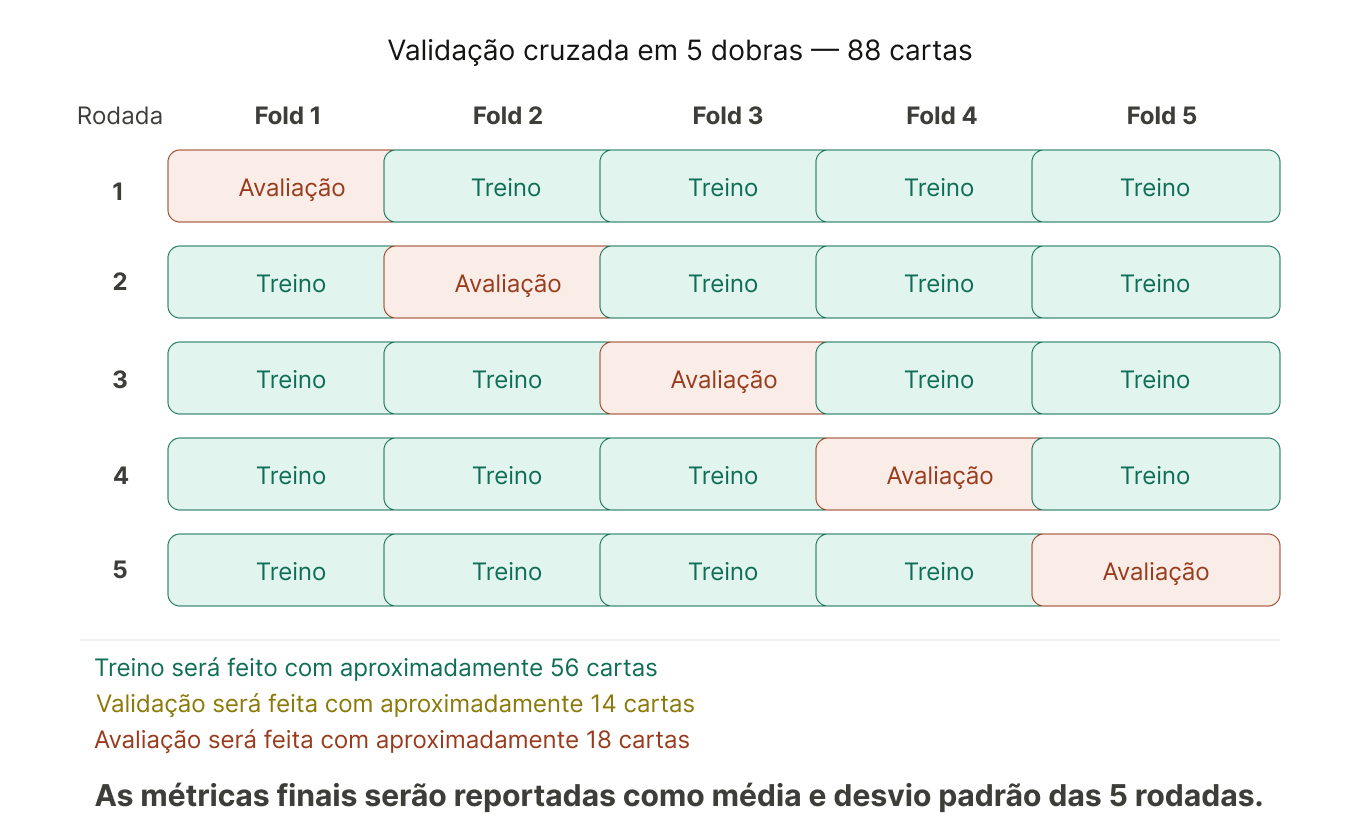
\includegraphics[width=1.00\textwidth]{imagens/kfold.png}
    \caption{Esquema da validação cruzada estratificada em cinco dobras 
    aplicada ao conjunto de 88 cartas. Em cada rodada, quatro folds são 
    utilizados para treinamento e um fold é reservado para avaliação, 
    mantendo frente e verso da mesma carta no mesmo fold. Do bloco de 
    treinamento de cada rodada, aproximadamente 20\% das cartas (~14) são 
    separadas aleatoriamente como \textit{validation set} para monitoramento 
    do \textit{early stopping}, permanecendo o fold de avaliação completamente 
    isolado durante o treinamento.}
    \fonte{Elaborado pelo autor (2026).}
    \label{fig:kfold_cross_validation}
\end{figure}

Considerando o baixo volume de dados disponível e a dificuldade 
associada à anotação de defeitos pequenos e visualmente sutis em cartas TCG,
a modelagem inicial do problema será realizada com uma única classe de interesse,
denominada \textit{defeito}. Em inspeção visual, a detecção de defeitos pode 
envolver informações como categoria, localização, contorno e tamanho da imperfeição
\cite{Chen2021}; no entanto, neste trabalho, opta-se por concentrar a avaliação 
na localização das regiões defeituosas, sem distinguir inicialmente os tipos 
específicos de dano.

As anotações do conjunto de dados serão produzidas pelo autor 
na forma de caixas delimitadoras (\textit{bounding boxes}) 
compatíveis com o formato YOLOv8, derivadas dos registros de 
defeitos identificados por avaliadores especializados em 
graduação de cartas TCG durante o processo de inspeção 
profissional. Esse tipo de anotação, fundamentada na avaliação 
de especialistas do domínio com critérios técnicos estabelecidos, 
é considerado o padrão de referência em tarefas de detecção de 
defeitos visuais \cite{Nahar2025}. A conversão dos registros 
de defeitos para o formato de detecção de objetos preserva a 
localização espacial das imperfeições identificadas pelos 
avaliadores, associando cada região defeituosa à classe única 
\textit{defeito}.

Essa decisão metodológica reduz a granularidade do problema, evita a 
fragmentação do conjunto de treinamento em múltiplas classes com poucos 
exemplos e favorece maior consistência nas anotações. Em inspeção visual 
automatizada com dados limitados, a redução do número de classes de 
detecção é uma estratégia reconhecida para preservar a representatividade 
dos exemplos disponíveis e melhorar a capacidade de generalização do 
modelo \cite{Chen2021}. Assim, no presente trabalho, o modelo não terá 
como objetivo diferenciar categorias como risco, dobra ou desgaste, 
mas sim identificar regiões da carta que apresentem indícios visuais 
de defeito.

\subsection{Modelo base}
\label{subsec:modelo_base}

Como modelo de detecção será utilizada a versão YOLOv8, selecionada por seu
equilíbrio entre eficiência computacional e desempenho em tarefas de detecção
de objetos. Considerando que o conjunto de dados disponível é reduzido e que
a classe de interesse, denominada \textit{defeito}, não faz parte das classes
originais do dataset COCO, todas as configurações experimentais partirão de
pesos pré-treinados e serão ajustadas ao domínio das cartas por meio de
\textit{fine-tuning}.

Neste trabalho, a configuração base (\textit{baseline}) corresponderá ao
YOLOv8 com \textit{transfer learning} treinado sobre as imagens RGB
convencionais, sem aumento de dados adicional e sem uso das imagens
fotométricas derivadas. Essa configuração servirá como referência para avaliar
a contribuição individual e combinada do aumento de dados.

Entre as variantes disponíveis do YOLOv8, todas pré-treinadas no 
dataset COCO \cite{Lin2014}, este trabalho adotará a versão 
\textit{small} (YOLOv8s), com aproximadamente 11 milhões de 
parâmetros. Essa escolha é motivada pela relação entre capacidade de 
representação e volume de dados disponível por fold: variantes maiores 
possuem dezenas de milhões de parâmetros adicionais que, com cerca de 
56 cartas de treinamento por rodada, aumentariam o risco de 
\textit{overfitting} mesmo com \textit{transfer learning}. 
\citeonline{Wang2022} demonstram, em contexto análogo de detecção de 
defeitos industriais com dados escassos, que modelos com maior número 
de parâmetros apresentam desempenho inferior a arquiteturas mais 
simples justamente por esse motivo. \citeonline{Dobrzycki2025} 
corroboram essa decisão ao verificar que, em cenários com dados 
limitados, variantes menores do YOLOv8 oferecem melhor equilíbrio 
entre desempenho e custo computacional do que variantes maiores. 
A adequação final da variante será confirmada nos testes preliminares 
previstos na Seção~\ref{subsec:hiperparametros}, nos quais YOLOv8n 
será avaliado como alternativa caso YOLOv8s apresente sinais de 
\textit{overfitting}.

Os demais experimentos partirão dessa configuração de referência e incorporarão
novas estratégias de forma controlada. Para garantir comparabilidade entre os
resultados, serão mantidos fixos, entre as configurações, parâmetros como
resolução de entrada, taxa de aprendizado, tamanho do lote, número máximo de
épocas e critério de parada antecipada. Assim, embora o número efetivo de épocas
possa variar entre os experimentos em função do \textit{early stopping}, todas
as configurações serão submetidas ao mesmo limite máximo de treinamento e à
mesma regra de interrupção. Esses valores serão definidos em testes preliminares
antes da execução do estudo de ablação.

\subsection{Hiperparâmetros de treinamento}
\label{subsec:hiperparametros}

Os hiperparâmetros de treinamento compreendem as configurações
do processo de otimização que não são aprendidas automaticamente
pelo modelo, sendo definidas pelo pesquisador antes do início
do treinamento \cite{Dobrzycki2025}. No presente trabalho, os
principais hiperparâmetros considerados são: taxa de aprendizado
(\textit{learning rate}), número de épocas, tamanho do lote
(\textit{batch size}), resolução de entrada das imagens e
critério de parada antecipada (\textit{early stopping}).

Os valores finais desses hiperparâmetros serão estabelecidos 
por meio de testes preliminares realizados sobre a configuração
base antes da execução do estudo de ablação. Uma vez definidos,
os mesmos valores serão mantidos fixos em todas as quatro configurações
experimentais. Essa decisão é essencial para garantir que as diferenças
de desempenho observadas entre as configurações sejam atribuíveis
exclusivamente às estratégias avaliadas, como o tipo de imagem e
o uso de aumento de dados, e não a variações no processo de otimização
\cite{Dobrzycki2025}.

O critério de parada antecipada será configurado para monitorar o 
mAP@0.5 em um subconjunto de validação interno (\textit{validation 
set}), constituído por aproximadamente 20\% das cartas do bloco de 
treinamento de cada rodada, correspondendo a cerca de 14 cartas (28 
imagens). Esse subconjunto é distinto do fold de avaliação, que 
permanece completamente isolado durante o treinamento e é utilizado 
exclusivamente para reportar o desempenho final de cada configuração 
experimental. A paciência inicial será de 50 épocas, valor compatível 
com o tamanho reduzido do conjunto de dados e alinhado aos padrões da 
biblioteca Ultralytics para YOLOv8 \cite{Dobrzycki2025}. O valor final 
da paciência será ajustado nos testes preliminares, sendo mantido fixo 
em todas as quatro configurações experimentais para garantir 
comparabilidade entre os resultados.

Como ponto de partida para os testes preliminares, 
serão adotados os valores padrão recomendados pela
biblioteca Ultralytics para o YOLOv8, ajustando-os
conforme necessário para o tamanho reduzido do 
conjunto de dados disponível. Adicionalmente,
os testes preliminares contemplarão a validação 
da variante do modelo, avaliando YOLOv8n como
alternativa a YOLOv8s caso sejam observados sinais
de \textit{overfitting}, bem como a definição dos
parâmetros do pipeline de pré-processamento fotométrico.
Esses parâmetros incluem o kernel do filtro emboss 
($3{\times}3$), o \textit{clipLimit} (valor de referência: 3,0)
e o \textit{tileGridSize} ($8{\times}8$ pixels) do CLAHE.
Todos os valores definidos nessa etapa serão mantidos fixos 
entre as quatro configurações experimentais, garantindo que
as diferenças de desempenho observadas sejam atribuíveis 
exclusivamente às estratégias avaliadas.


\subsection{Estratégias de treinamento avaliadas}
\label{subsec:estrategias}

O trabalho comparará quatro configurações experimentais baseadas
em YOLOv8 com \textit{transfer learning}, variando de forma
controlada duas estratégias: o uso de aumento de dados
(\textit{data augmentation}) e o tipo de representação visual
da entrada, que pode ser a imagem RGB convencional ou a imagem
fotométrica derivada gerada. Esse
desenho permite avaliar a contribuição individual e combinada
de cada estratégia no desempenho do detector em um cenário
com baixo volume de dados.

O \textit{transfer learning} será empregado em todas as configurações por meio 
do ajuste fino (\textit{fine-tuning}) de pesos pré-treinados, buscando aproveitar 
representações visuais previamente aprendidas em bases de larga escala. Essa 
decisão é justificada pelo baixo volume de dados disponível e pela necessidade 
de adaptar o detector à classe de interesse \textit{defeito}, inexistente nas 
classes originais do COCO. Dessa forma, o \textit{transfer learning} não será 
tratado como uma variável comparativa isolada no estudo de ablação, mas como 
a base comum de treinamento sobre a qual serão avaliados o aumento de dados 
e o uso de imagens fotométricas derivadas.

O aumento de dados será utilizado para ampliar artificialmente a variabilidade 
do conjunto de treinamento. Para a representação RGB, serão aplicadas transformações
geométricas (flip horizontal, rotação de até ±10°) e fotométricas (variação de brilho e saturação).
Para a representação fotométrica, serão utilizadas apenas transformações geométricas, uma vez que a
imagem embossada já passou por normalização via CLAHE, tornando inconsistente a aplicação de variações artificiais de brilho ou contraste.

Já o uso das imagens fotométricas derivadas será avaliado como uma 
representação alternativa de entrada, com o objetivo de verificar se 
o realce de textura, relevo e irregularidades superficiais contribui 
para a detecção de defeitos visuais. Essas imagens serão geradas pela 
aplicação sequencial de filtro emboss e CLAHE sobre as imagens RGB 
originais, utilizando a biblioteca OpenCV. O filtro emboss utiliza um 
kernel direcional $3{\times}3$ fixo, e o CLAHE é configurado com 
\textit{clipLimit} inicial de 3,0 e \textit{tileGridSize} de 
$8{\times}8$ pixels, valores de referência adotados como ponto de 
partida nos testes preliminares previstos na 
Seção~\ref{subsec:hiperparametros}, nos quais serão avaliados 
empiricamente e mantidos fixos entre todas as configurações 
experimentais após definição.

\subsection{Estudo de ablação}
\label{subsec:ablacao}

A comparação entre as estratégias será realizada por meio de um
estudo de ablação com desenho fatorial. Nesse tipo de desenho,
duas variáveis independentes, o uso de aumento de dados e o
tipo de representação visual da entrada são combinadas de
forma controlada, permitindo avaliar a contribuição individual
e conjunta de cada estratégia no desempenho do detector.

Serão consideradas quatro configurações experimentais:

\begin{enumerate}
    \item YOLOv8 com \textit{transfer learning} em imagens RGB;
    \item YOLOv8 com \textit{transfer learning} e aumento de dados 
    em imagens RGB;
    \item YOLOv8 com \textit{transfer learning} em imagens 
    fotométricas derivadas;
    \item YOLOv8 com \textit{transfer learning} e aumento de dados 
    em imagens fotométricas derivadas.
\end{enumerate}

A configuração 1 serve como referência do estudo de ablação,
correspondendo ao cenário mais simples: fine-tuning com imagens
RGB sem aumento de dados. As demais configurações introduzem
variações controladas sobre essa referência, mantendo fixos
os hiperparâmetros de treinamento em todas as configurações
para garantir que as diferenças de desempenho observadas sejam
atribuíveis exclusivamente às estratégias avaliadas.

Os folds serão definidos uma única vez sobre as 88 cartas e mantidos
fixos entre todas as configurações, de modo que cada configuração seja
avaliada exatamente sobre as mesmas partições. A comparação entre
as quatro estratégias será feita com base no mAP@0.5 médio sobre
as cinco rodadas, com o desvio padrão utilizado para avaliar a
consistência dos resultados \cite{Kohavi1995}.

Esse desenho foi escolhido por ser compatível com o escopo do TCC1 e por 
permitir uma análise clara da influência de cada estratégia em um contexto 
de baixo volume de dados. Em vez de comparar múltiplas arquiteturas, a proposta 
fixa o modelo YOLOv8 e concentra a investigação naquilo que constitui a 
contribuição principal do trabalho: a comparação entre estratégias de treinamento.

\subsection{Tecnologias e ferramentas}
\label{subsec:ferramentas}

A implementação será realizada em Python. Para o treinamento do 
modelo, será utilizada a biblioteca oficial da família YOLOv8. O processamento 
das imagens e as etapas de preparação do conjunto de dados poderão ser apoiados 
por bibliotecas de manipulação de imagens e visão computacional, como OpenCV. 
Para a aplicação de transformações de aumento de dados, poderão ser utilizadas 
bibliotecas específicas de \textit{augmentation}, desde que compatíveis com o 
pipeline definido.

Os experimentos serão executados em ambiente computacional com suporte a GPU, 
de modo a reduzir o tempo de treinamento e viabilizar a execução das diferentes 
configurações previstas no estudo de ablação.

\subsection{Critérios de validação}
\label{subsec:validacao}

A validação do desempenho do modelo será feita por meio de métricas quantitativas 
utilizadas em tarefas de detecção de objetos. A métrica principal será o 
\textit{mean Average Precision} com limiar de IoU de 0,5 (mAP@0.5), por permitir 
uma visão sintética do desempenho do detector em termos de classificação e localização.

Como métricas complementares, também serão utilizados precisão, \textit{recall} 
e F1-score, com o objetivo de fornecer uma análise mais detalhada do comportamento 
do modelo em cada configuração experimental. Em razão do baixo volume de dados, 
os resultados serão reportados como média e desvio padrão sobre as cinco rodadas 
da validação cruzada, tornando a comparação entre estratégias mais robusta do que 
uma única avaliação permitiria \cite{Kohavi1995, Wang2022}. A comparação entre os 
experimentos buscará identificar quais estratégias produzem ganhos mais consistentes 
no cenário de dados limitados considerado neste trabalho.

% ---------------------------------------------------------------
\section{Cronograma de trabalho}
\label{sec:cronograma}

O cronograma de trabalho organiza as principais atividades previstas para o desenvolvimento do TCC2, contemplando desde a preparação final do conjunto de dados até a execução dos experimentos, análise dos resultados e redação da versão final do trabalho. As etapas foram distribuídas de forma sequencial, considerando a dependência entre a organização dos dados, o treinamento dos modelos, a comparação das configurações experimentais e a consolidação dos resultados obtidos.

\begin{figure}[htb]
    \centering
    \captionsetup{justification=centering}
    \caption{Cronograma de atividades do TCC2 para o segundo semestre de 2026 -- Diagrama de Gantt}
    \label{fig:gantt}

    \begin{ganttchart}[
        hgrid,
        vgrid,
        x unit=0.68cm,
        y unit title=0.6cm,
        y unit chart=1cm,
        title height=1,
        bar height=0.45,
        bar label font=\scriptsize,
        group label font=\scriptsize\bfseries,
        title label font=\small,
        milestone label font=\scriptsize\itshape,
        bar/.append style={fill=blue!40},
        group/.append style={draw=black, fill=blue!70},
        milestone/.append style={fill=red!70},
        bar label node/.append style={text width=3.8cm, align=right},
        group label node/.append style={text width=3.8cm, align=right},
        milestone label node/.append style={text width=3.8cm, align=right}
    ]{1}{16}
        \gantttitle{Segundo semestre de 2026}{16} \\
        \gantttitle{Semanas}{16} \\
        \gantttitlelist{1,...,16}{1} \\

        \ganttgroup{Fase 1: Preparação experimental}{1}{4} \\
        \ganttbar{Revisão da literatura e metodologia}{1}{2} \\
        \ganttbar{Revisão das anotações do dataset}{2}{4} \\
        \ganttbar{Particionamento dos dados}{3}{4} \\
        \ganttmilestone{Base preparada}{4} \\

        \ganttgroup{Fase 2: Implementação do pipeline}{5}{7} \\
        \ganttbar{Configuração do ambiente}{5}{5} \\
        \ganttbar{Implementação do YOLOv8 base}{5}{6} \\
        \ganttbar{Ajuste de hiperparâmetros}{6}{7} \\
        \ganttmilestone{Pipeline validado}{7} \\

        \ganttgroup{Fase 3: Execução dos experimentos}{8}{13} \\
        \ganttbar{Exp. 1: RGB sem augmentation}{8}{8} \\
        \ganttbar{Exp. 2: RGB com augmentation}{9}{10} \\
        \ganttbar{Exp. 3: Fotométrica sem augmentation}{10}{11} \\
        \ganttbar{Exp. 4: Fotométrica com augmentation}{11}{12} \\
        \ganttbar{Comparação dos resultados}{12}{13} \\
        \ganttmilestone{Ablação concluída}{13} \\

        \ganttgroup{Fase 4: Redação e finalização}{14}{16} \\
        \ganttbar{Resultados e discussão}{14}{15} \\
        \ganttbar{Revisão final do TCC2}{15}{16} \\
        \ganttmilestone{Entrega final}{16}
    \end{ganttchart}

    \legend{Fonte: Elaborado pelo autor (2026)}
\end{figure}



% ---------------------------------------------------------------
% ELEMENTOS PÓS-TEXTUAIS
% ---------------------------------------------------------------
\postextual

% ===============================================================
% CAPÍTULO 4 - REFERÊNCIAS BIBLIOGRÁFICAS
% ===============================================================
\bibliography{bibliografia}

\end{document}